\documentclass[a4paper,11pt,reqno]{amsart}

% --------------------------------------------------------
% Packages
% --------------------------------------------------------
\usepackage[utf8]{inputenc}
\usepackage[foot]{amsaddr}
\usepackage{amsmath,amsfonts,amssymb,amsthm,mathrsfs,bm}
\usepackage[margin=0.95in]{geometry}
\usepackage{color}
\usepackage[dvipsnames]{xcolor}
\usepackage{mathtools,graphicx}
\usepackage{tcolorbox}
\usepackage{listings}
\usepackage{textcomp}
\usepackage{hyperref}

% --------------------------------------------------------
% Custom Colours
% --------------------------------------------------------
\definecolor{CommentGreen}{rgb}{0.0,0.4,0.0}
\definecolor{Background}{rgb}{0.9,1.0,0.85}
\definecolor{lrow}{rgb}{0.914,0.918,0.922}
\definecolor{drow}{rgb}{0.725,0.745,0.769}


% --------------------------------------------------------
% Typesetting Python code
% --------------------------------------------------------
\lstloadlanguages{Python}%
\lstset{
    language=Python, upquote=true, frame=single,
    basicstyle=\small\ttfamily,
    backgroundcolor=\color{yellow!30},
    keywordstyle=[1]\color{NavyBlue}\bfseries,
    keywordstyle=[2]\color{RubineRed},
    keywordstyle=[3]\color{orange!90}\bfseries,
    keywordstyle=[4]\color{Green!90}\bfseries,
    identifierstyle=,
    commentstyle=\usefont{T1}{pcr}{m}{sl}\color{MidnightBlue}\small,
    stringstyle=\color{purple},
    showstringspaces=false, tabsize=4, morekeywords={import,as},
    morekeywords=[2]{args,__init__},
    morekeywords=[3]{@property},
    morekeywords=[4]{self},
    morecomment=[l][\color{blue}]{...},
    numbers=none, firstnumber=1,
    numberstyle=\tiny\color{blue},
    stepnumber=1, xleftmargin=10pt, xrightmargin=10pt
}

\synctex=1

\hypersetup{
    unicode=false, pdftoolbar=true, 
    pdfmenubar=true, pdffitwindow=false, pdfstartview={FitH}, 
    pdftitle={ELE2024 Coursework}, pdfauthor={A. Author},
    pdfsubject={ELE2024 coursework}, pdfcreator={A. Author},
    pdfproducer={ELE2024}, pdfnewwindow=true,
    colorlinks=true, linkcolor=red,
    citecolor=blue, filecolor=magenta, urlcolor=cyan
}

% --------------------------------------------------------
% CUSTOM COMMANDS
% --------------------------------------------------------
\renewcommand{\Re}{\mathbf{re}}
\renewcommand{\Im}{\mathbf{im}}
\newcommand{\R}{\mathbb{R}}
\newcommand{\N}{\mathbb{N}}
\newcommand{\C}{\mathbb{C}}
\newcommand{\lap}{\mathscr{L}}
\newcommand{\dd}{\mathrm{d}}
\newcommand{\smallmat}[1]{\left[ \begin{smallmatrix}#1 \end{smallmatrix} \right]}

% --------------------------------------------------------
% Opening: Title and Author Names
%          Modify this section
% --------------------------------------------------------
\title[ELE2024 Coursework]{Report for the ELE2024 coursework}

\author[B. Harkin]{Ben Harkin}
\author[D. Lim]{David Lim}
\author[C. Watts]{Cerys Watts}
\address[B. Harkin, D. Lim and C. Watts]{Email addresses: \href{mailto:bharkin02@qub.ac.uk} {bharkin02@qub.ac.uk}, \href{mailto:dlim04@qub.ac.uk}{dlim04@qub.ac.uk} and \href{mailto:cwatts06@qub.ac.uk}{cwatts06@qub.ac.uk}.}
\thanks{Some note goes here.  Version 0.0.1. Last updated:~\today.}



% --------------------------------------------------------
% Beginning of your document
% --------------------------------------------------------
\begin{document}

\maketitle


\section{Part A: Control Theory}
\subsection*{Given Equations} The following equations were given by Dr P. Soposakis as part of the coursework brief:

\begin{equation} \label{eq:1}
    L = L_0 + L_1 \exp{(-\alpha y)}
\end{equation}

\begin{equation} \label{eq:2}
    F_{mag}=c \frac{I^2}{y^2}
\end{equation}

  \hspace{6cm} where y = $\delta$ - x \\
This is the diagram that we have used:\\
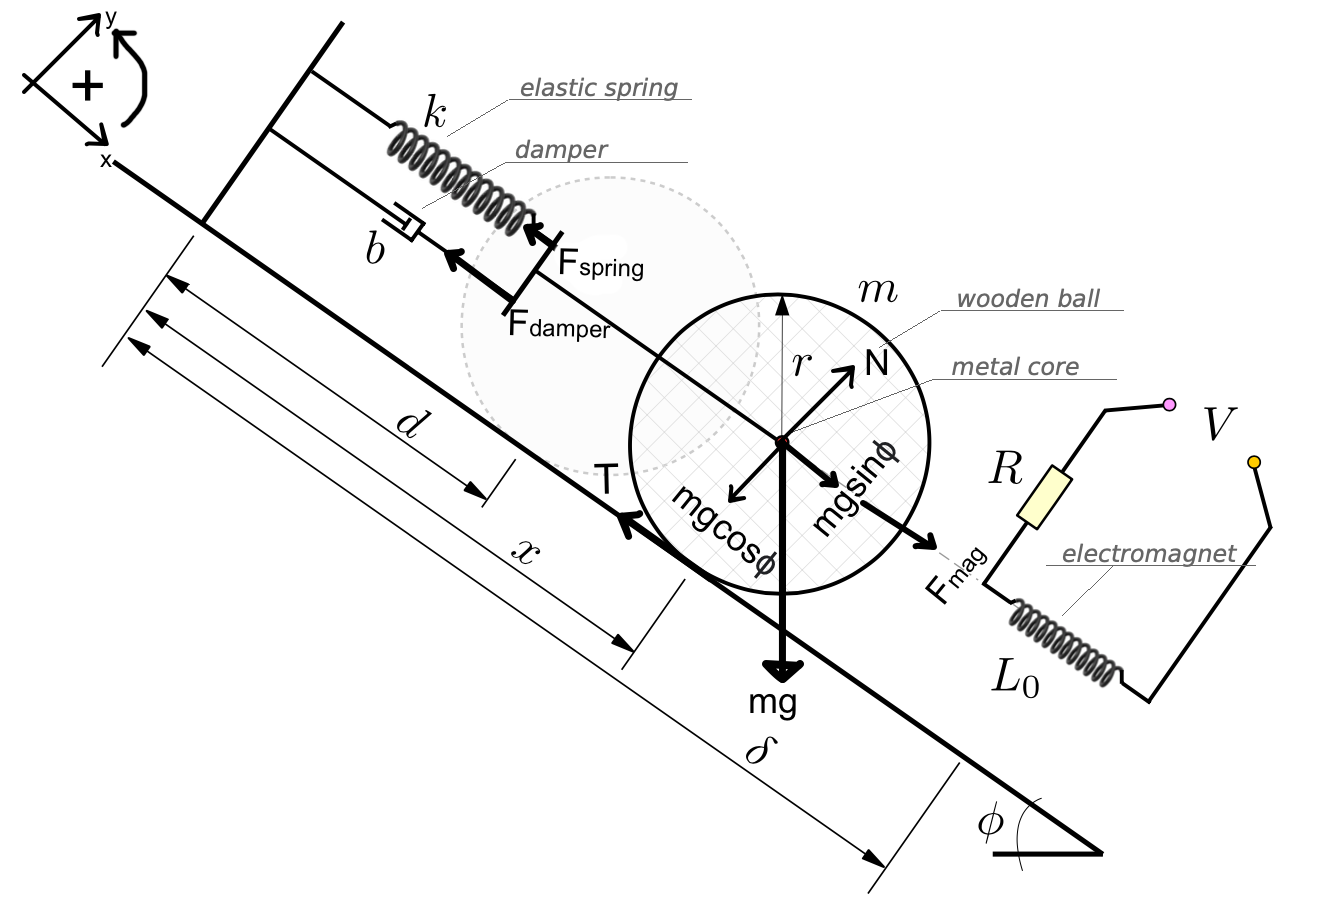
\includegraphics[scale=0.6]{Report/figures/main_diagram}
    \subsection*{Problem A1}
\hfill \break
\begin{figure}[h!]
  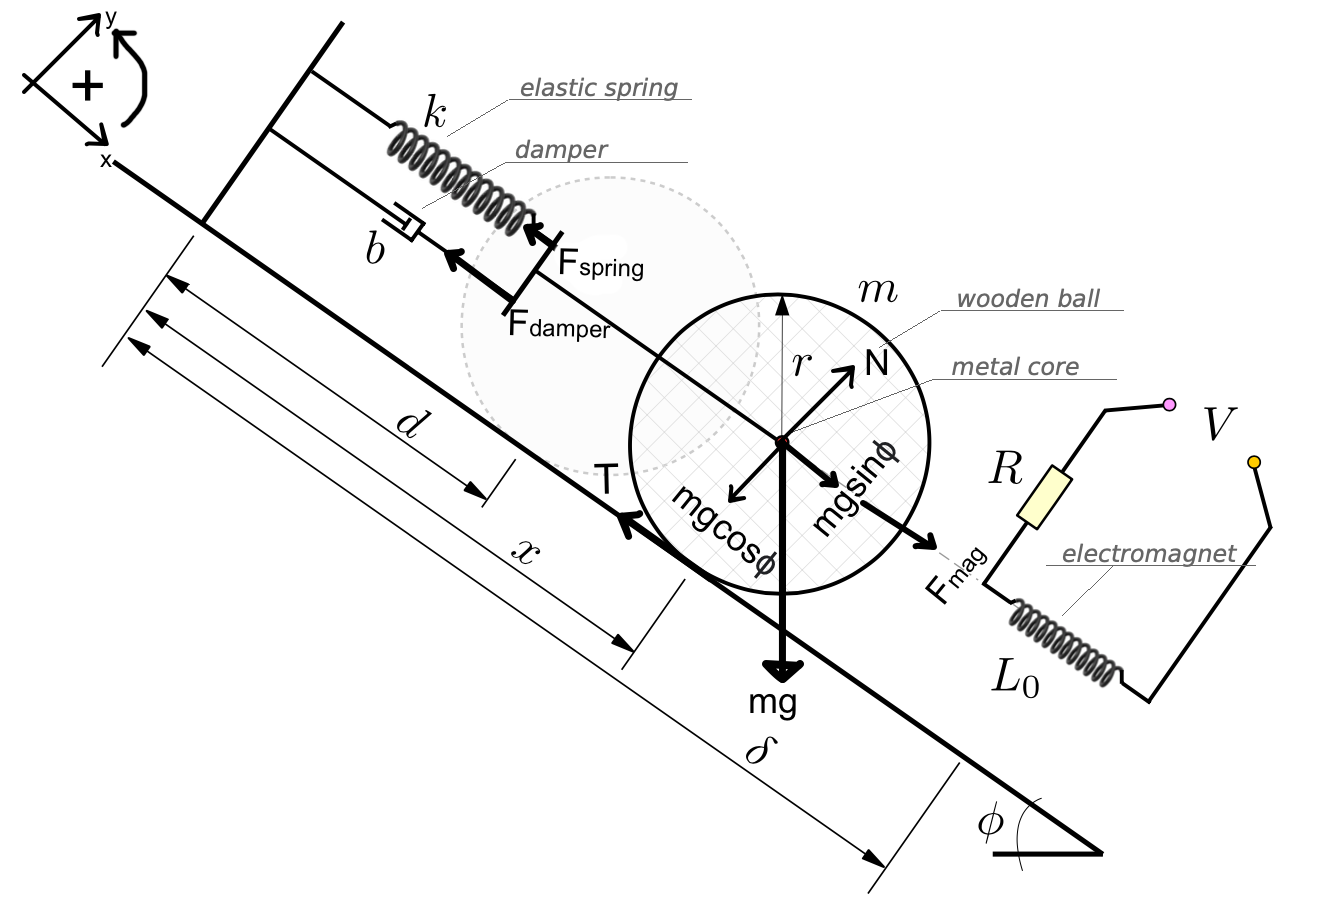
\includegraphics[width=0.7\textwidth]{Report/figures/main_diagram}
  \caption{System of a wooden ball on n inclined plane that can be attracted by an electromagnet, controlled by a voltage V, with forces applied labelled.}
  \label{fig:system}
\end{figure}

    \begin{align}
        F_{spring} &= k(x - d)\label{eq:3}\\
        F_{damper} &= b\dot{x}\label{eq:4}
    \end{align}
    \begin{equation} \label{eq:5}
        Tr &= -I\ddot{\theta} \therefore T = -\frac{I\ddot{\theta}}{r}
    \end{equation}
    \begin{align} 
        I &= \frac{2}{5} mr^2 \label{eq:6} \\
        \ddot{\theta} &= \frac{\ddot{x}}{r} \label{eq:7} \\\nonumber
    \end{align}
    Sub \eqref{eq:6} and \eqref{eq:7} into \eqref{eq:5}:
    \begin{equation} \label{eq:8}
        T = -\frac{2m\ddot{x}}{5}
    \end{equation}
    Apply Newtons 2nd Law of Motion to the system: 
    \begin{equation} \label{eq:9}
        F_{mag} + mg \sin{\phi} - T - F_{spring} - F_{damper} &= m \ddot{x}
    \end{equation}
    Sub \eqref{eq:2}, \eqref{eq:3}, \eqref{eq:4} and \eqref{eq:8} into \eqref{eq:9}:
    \begin{align} 
       \frac{cI^2}{y^2} + mg \sin{\phi} + \frac{2m \ddot{x}}{5} - k(x - d) - b \dot{x} &= m \ddot{x} \nonumber \\
       \text{(ODE)}\frac{cI^2}{(\delta - x)^2} + mg \sin{\phi} - k(x -d) - b \dot{x} &= \frac{3m}{5} \ddot{x}\label{eq:10}
    \end{align}
    Apply Kirchoff's Voltage Law to system circuit:
    \begin{align}
        V &= V_{R} + V_{L} \label{eq:11} \\
        V_{R} &= IR\label{eq:12}\\
        V_{L} &= L \dot{I}\label{eq:13}
    \end{align}
    Sub \eqref{eq:12}, \eqref{eq:13} into \eqref{eq:11}: 
    \begin{equation} \label{eq:14}
        V &= IR + L\dot{I}
    \end{equation}
    Sub \eqref{eq:1} into \eqref{eq:14}: 
    \begin{equation} \label{eq:15}
        \text{(ODE)}V &= IR + (L_0 + L_1 \exp{(-\alpha y)})\dot{I}
    \end{equation}
    \hfill \break
    Equations \eqref{eq:10} and \eqref{eq:15} are the ordinary differential equations for the system shown in Figure 1.
    
    
    
    
    \subsection*{Problem A2}
    Write the system you determined in Problem A1 in a state space representation. What are the states and inputs of the system?

    \begin{align}
        V &= IR + (L_{0} + L_{1} ^{- \alpha (d - x)})\dot{I}
    \end{align}
    \begin{align}
        I_1 &= I\nonumber\\
        \therefore \dot{I} &= \dot{I_1}\nonumber\\
        V &= IR + (L_{0} + L_{1} ^{- \alpha (d - x)})\dot{I}\nonumber\\
        V &= IR + (L_{0} + L_{1} ^{- \alpha (d - x)})\dot{I_1}\nonumber\\
        V - IR &= (L_{0} + L_{1} ^{- \alpha (d - x)})\dot{I_1}\nonumber\\
        V - IR &= (L_{0} + L_{1} ^{- \alpha (d - x)})\dot{I_1}\nonumber\\
        \therefore
        \dot{I} &= \frac{V - IR}{(L_{0} + L_{1} ^{- \alpha (d - x)})}
    \end{align}


    \begin{align}
        \frac{c I^2}{(d - x)^2} + mg \sin{\phi} - k(x -d) - b \dot{x} &= \frac{3m}{5} \ddot{x} \\
        x_1 = x, x_2 = \dot{x_1}, \therefore \ddot{x} = \dot{x_2}\nonumber\\
        \bm{x} =
        \begin{bmatrix}
            x_1
            \\
            x_2
        \end{bmatrix}
        \therefore \bm{\dot{x}} =
        \begin{bmatrix}
            \dot{x_1}
            \\
            \dot{x_2}
        \end{bmatrix} \nonumber
    \end{align}
    \begin{align}
        \frac{c I^2}{(d - x)^2} + mg \sin{\phi} - k(x -d) - b \dot{x} &= \frac{3m}{5} \dot{x_2} \nonumber\\
        \frac{5(\frac{c I^2}{(d - x)^2} + mg \sin{\phi} - k(x -d) - b \dot{x})}{3m} &= \dot{x_2} \nonumber
    \end{align}
    \begin{align}
        \therefore \bm{\dot{x}} &=
        \begin{bmatrix}
            x_2
            \\
            \frac{5(\frac{c I^2}{(d - x)^2} + mg \sin{\phi} - k(x -d) - b \dot{x})}{3m}
            \\
            \frac{V - IR}{(L_{0} + L_{1} ^{- \alpha (d - x)})}
        \end{bmatrix}
    \end{align}





    \subsection*{Problem A3} 
\hfill \break
According to Proposition 3.4 in the textbook
    \subsection*{Problem A4} 
    \hfill \break
    Subtract by parts Equations \eqref{eq:16} and \eqref{eq:18}:
    \begin{align}
        \dot{x_1} = x_2 \nonumber\\ 
        \text{--- } \hspace{0.5cm} 0 = x^e \nonumber \\
        \hspace{3cm}\rule{3cm}{1pt} \nonumber \\
        \therefore \dot{\bar{x}} = x_2 - x_2^e \nonumber \\
        = \bar{x_2} \nonumber
    \end{align}
    \hfill \break
    \begin{align}
        \dot{x_2} = \frac{5cI^2}{3m(\delta - x_1)^2} + \frac{5g\sin{\phi}}{3} - \frac{5k}{3m}(x_1 -d) - \frac{5b x_2}{3m}\nonumber\\ 
        \text{--- }  \hspace{2cm}0 = \frac{5cI^e^2}{3m(\delta - x_1^e)^2} + \frac{5g\sin{\phi}}{3} - \frac{5k}{3m}(x_1^e -d)  \nonumber \\
        \rule{10cm}{1pt} \nonumber \\
        \dot{\bar{x_2}} ={\frac{5c}{3m}\left( \frac{I^2}{(\delta -{x_1})^2} -  \frac{I^e^2}{(\delta -{x_1^{e}})^2}\right)}-{\frac{5k}{3m}{(x_1 - x_1^e)}}-{\frac{5b}{3m}x_2} \label{eq:20}
    \end{align}
    \hfill \break
    Apply Taylor's Theorem to Equation \eqref{eq:20}:
    \begin{align}
        g(I, x_1) \approx g(I^e, x_1^e) + \frac{\partial g}{\partial I_{I^e, x_1^e}}\cdot (I - I^e) + \frac{\partial g}{\partial x_{I^e, x_1^e}}\cdot (x_1 - x_1^e) \label{eq:21}
    \end{align}
    \begin{align}
        g(I, x_1) = \frac{I^2}{(\delta - x_1)^2} \label{eq:22}\\
        \frac{\partial g}{\partial I} = \frac{2I}{(\delta -{x_1})^2}\label{eq:23} \\
        \frac{\partial g}{\partial x_1} = \frac{2I^2}{(\delta -{x_1})^3} \label{eq:24}
    \end{align}
    Sub Equations \eqref{eq:22},\eqref{eq:23} and \eqref{eq:24} into \eqref{eq:21}:
    \begin{align}
         \frac{I^2}{(\delta - x_1)^2} = \frac{I^e^2}{(\delta - x_1^e)^2} + \frac{2I^e}{(\delta -{x_1^e})^2}\cdot (I - I^e) + \frac{2I^e^2}{(\delta -{x_1^e})^3}\cdot (x_1 - x_1^e) \nonumber \\
         \frac{I^2}{(\delta - x_1)^2} - \frac{I^e^2}{(\delta - x_1^e)^2} = \frac{2I^e}{(\delta -{x_1^e})^2}\cdot (I - I^e) + \frac{2I^e^2}{(\delta -{x_1^e})^3}\cdot (x_1 - x_1^e)  \label{eq:25}
    \end{align}
    Sub Equation \eqref{eq:25} into Equation \eqref{eq:20}:
    \begin{equation}
         \dot{\bar{x_2}} = \frac{5c}{3m}\left( \frac{2I^e}{(\delta -{x_1^e})^2}\cdot (I - I^e) + \frac{2I^e^2}{(\delta -{x_1^e})^3}\cdot (x_1 - x_1^e)\right) - \frac{5k}{3m}(x_1 - x_1^e) - - \frac{5b}{3m}(x_2) \label{eq:26}
    \end{equation}
    Introduce deviation variables:
    \begin{align}
         \bar{I} &= I - I^e \nonumber\\
         \bar{x_1} &= x_1 - x_1^e \nonumber\\
         \bar{x_2} &= x_2 - x_2^e = x_2 - 0 = x_2 \nonumber
    \end{align}
    to Equation \eqref{eq:26}:
    \begin{align}
         \dot{\bar{x_2}} = \frac{5c}{3m}\left( \frac{2I^e}{(\delta -{x_1^e})^2}\cdot \bar{I} + \frac{2I^e^2}{(\delta -{x_1^e})^3}\cdot \bar{x_1}\right) - \frac{5k}{3m}(\bar{x_1}) - \frac{5b}{3m}(\bar{x_2}) \nonumber \\
         \dot{\bar{x_2}} =\frac{5c2I^e}{(3m\delta -{x_1^e})^2}\cdot \bar{I} + \frac{10cI^e^2}{3m(\delta -{x_1^e})^3}\cdot \bar{x_1} - \frac{5k}{3m}(\bar{x_1}) - \frac{5b}{3m}(\bar{x_2}) \nonumber \\
         \dot{\bar{x_2}} =\frac{5c2I^e}{(3m\delta -{x_1^e})^2}\cdot \bar{I} + \left(\frac{10cI^e^2}{3m(\delta -{x_1^e})^3} - \frac{5k}{3m}\right)(\bar{x_1}) - \frac{5b}{3m}(\bar{x_2}) \label{eq:27} 
    \end{align}
    For Equation \eqref{eq:27}, let :
    \begin{equation}
         a =\frac{5c2I^e}{(3m\delta -{x_1^e})^2}, b = \left(\frac{10cI^e^2}{3m(\delta -{x_1^e})^3} - \frac{5k}{3m}\right) c = \frac{5b}{3m} \nonumber
    \end{equation}
    Subtract by parts \eqref{eq:17} and \eqref{eq:19} :
    \begin{align}
        {\dot{I}} = \frac{V - {I_1}R}{\left(L_{0} + L_{1}\exp{- \alpha y}\right)}\nonumber\\ 
        \text{--- }  0 = \frac{V^e - {I_1^e}R}{\left(L_{0} + L_{1}\exp{- \alpha (d - x)}\right)} \nonumber \\
        \rule{6cm}{1pt} \nonumber \\
        {\dot{\bar{I}}} = \frac{V - V^e - {I_1}R- {I_1^e}R}{\left(L_{0} + L_{1}\exp{- \alpha y}\right)}\label{eq:28}
    \end{align}
    Introduce deviation variables,
    \begin{align}
        \bar{V} = V - V^e \nonumber \\
        \bar{I} = I_1 - I_1^e \nonumber
    \end{align}
    to Equation \eqref{eq:28}:
    \begin{equation}\label{eq:29}
        \dot{\bar{I}} = \frac{\bar{V} - \bar{I_1}R}{\left(L_{0} + L_{1}\exp{- \alpha y}\right)}
    \end{equation}
    \hfill \break \\
    Let $f = {L_{0} + L_{1}\exp{(- \alpha y)}}$ for Equation \eqref{eq:29}\\
    \hfill \break \\
    The Linearised system equations are: \\
    \begin{align}
        \dot{\bar{x}} &= \bar{x_2}\label{eq:30} \\
        \dot{\bar{x_2}} &= a\bar{I} + b\bar{x_1} -c\bar{x_2}\label{eq:31} \\
        \dot{\bar{I}} &= \frac{1}{f}(\bar{V} - \bar{I}R)\label{eq:32}
    \end{align}
    \subsection*{Problem A5}Determine the transfer function of the linearised system that you determined in Problem A4. The input of the system is the voltage across the circuit and the output is the position of the ball on the inclined plane. How many poles does this transfer function have? Derive sufficient conditions on the system parameters under which the impulse response of the transfer function is oscillatory.

    
\section{Part B: Analysis and Controller Design}
    \subsection*{Problem B1}
\hfill \break
The wooden ball is limited to where it can equilibrate  by the physical limits of the system.\\
$x_{max}$ is the point furthest down the slope where the ball can equilibrate. This cannot be any further down the slope than the location of the electromagnet. This location is denoted on Figure \ref{fig:system} with $\delta$.\\
$\therefore$ We can say that $x_{max}$ can be no greater than $\delta$.\\
The limit of where the ball could equilibriate on the upper end of the slope is denoted by $x_{min}$. $d$ is the natural length of the spring, so $x_{min}$ can be no less than that, but we also need to take into account the downward force of the ball. This downward force is denoted in Figure \ref{fig:system} with $mg\sin{\phi}$. \\
However, the ball is not free to roll unobstructed. Taking into account the stiffness of the spring $k$, we can see that $x_{min}$ can be no smaller than $d + \frac{mg\sin{\phi}}{k}$.\\
$\therefore$ We can say that the system can only equilibrate at those positions $x^e$ that satisfy: \\
\begin{equation}
    d + \frac{mg\sin{\phi}}{k} < x^e < \delta
\end{equation}
To calculate the equilibrium voltage and current we use Equation \eqref{eq:10}. 
\begin{equation} \nonumber
    \frac{cI^2}{(\delta - x)^2} + mg \sin{\phi} - k(x -d) - b \dot{x} &= \frac{3m}{5} \ddot{x}
\end{equation}
To equilibriate, velocity and acceleration are equal to zero: \\
\begin{align} 
    \therefore \frac{cI^2}{(\delta - x)^2} + mg \sin{\phi} - k(x -d)  = 0 \nonumber \\
    \frac{-cI^2}{(\delta - x)^2} = mg \sin{\phi} - k(x -d) \nonumber \\
    \therefore I^e = \sqrt{\frac{(mg\sin{\phi}) - k(x_1^e - d)}{-c}(\delta - x_1^e)^2}
\end{align}
\begin{align} 
    V^e &= I^e \cdot R \nonumber \\
    \therefore V^e &= \left(\sqrt{\frac{(mg\sin{\phi}) - k(x_1^e - d)}{-c}(\delta - x_1^e)^2} \right) R
\end{align}
    \subsection{Problem B2}

    \subsection*{Problem B3}
\hfill \break

  
    \subsection*{Problem B4}
    \hfill \break
    A simulation was run to determine the low-frequency and high-frequency asymptotes of the magnitude and phase lag of the transfer function of the linearised system. This simulation was written in Python for which the code can be found \href{https://github.com/drlim2u/ELE2024-Control-Coursework/blob/059953dc7b2d8ba0a86b6f437153ceb4442b7a60/PartB.py#L125}{here} and which produced the Figure \ref{fig:problem_b4} below.
    \begin{figure}[H]
        \centering
        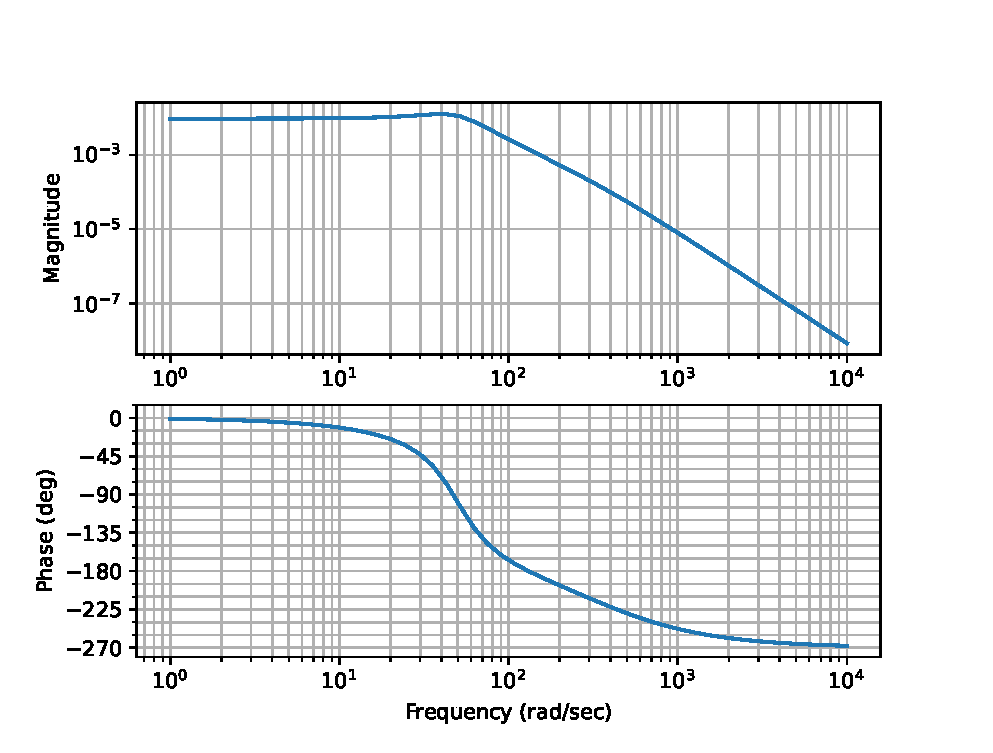
\includegraphics[width=0.6\linewidth]{figures/problem_b4.eps}
        \caption{Graphs showing both low-frequency and high-frequency asymptotes of the magnitude and phase lag of the transfer function of the linearised system.}
        \label{fig:problem_b4}
    \end{figure}
    \subsection{Problem B5}

    \subsection*{Problem B6}
    \hfill \break
    To control the system a Proportional Integral Differential (PID) controller was designed. The integral part of the PID controller will adjust for physical boundaries of the system and account for systematic errors and hopefully reduce and remove offset. This helps achieve the desired characteristic set out in Problem B5. The controller was written in Python and the implementaion can be found \href{https://github.com/drlim2u/ELE2024-Control-Coursework/blob/059953dc7b2d8ba0a86b6f437153ceb4442b7a60/PartB.py#L187}{here}. The step response from the simulated controlled system was recorded and is shown below in Figure \ref{fig:problem_b6}.
    
    \begin{figure}[H]
        \centering
        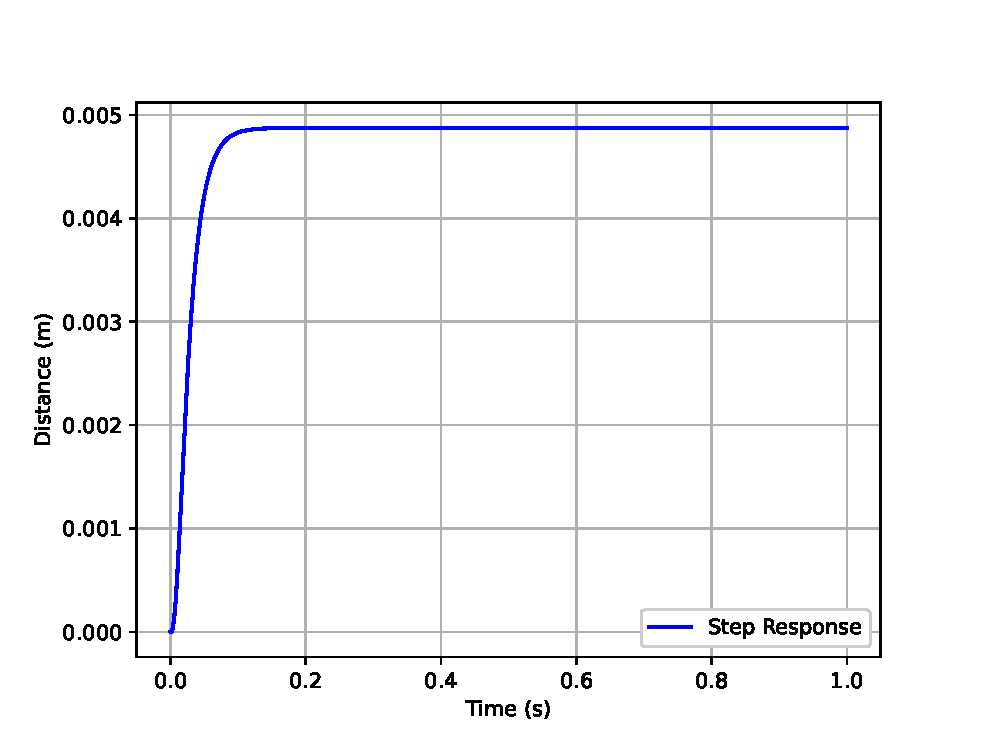
\includegraphics[width=0.6\linewidth]{figures/problem_b6.eps}
        \caption{Graph to show the step response of the system with a PID controller implemented.}
        \label{fig:problem_b6}
    \end{figure}
    
    As Figure \ref{fig:problem_b6} shows the system's impulse response settles very quickly.

    
\section{Part C: Bonus Questions}
    \subsection{Problem C1}

    \subsection{Problem C2} Determine the Laplace transform of f(t) = \(\left|{\cos{\left(\omega \right)}}\right|)\), \(t \geq 0\), \(\omega > 0\).

    \medskip
    The solution is:

    \smallskip
     \(\left( \frac{\left|{\cos{\left(\omega \right)}}\right|}{\omega}, \  0, \  \text{True}\right)\)

    \subsection{Problem C3}


\section{Part D: Planning, Organisation \& Collaboration}
    \subsection{D1}
    %***ALL OF THESE WILL BE UPDATED __JUST SOME IDEAS***
    We used a Github repository to collaborate on writing code. We used the git issue tracker to keep track of the tasks we were assigned and how those tasks were progressing. Here is the link to the issue tracker \href{https://github.com/drlim2u/ELE2024-Control-Coursework/issues}{here}.
    \subsection{D2}
    \subsubsection{Communication} We communicated clearly
    \subsubsection{Organisation} We began early and kept on top of our work.
    \subsubsection{Education} We all taught each other new things. etc

    \subsection{D3}
    The restrictions that exist due to Covid-19 was the main challenge presented to us. The fact that we were physically apart meant communication was limited to calls, texts and emails. Because these forms of communication are inherently more limited than face-to-face conversing it was important that we we communicate, we clearly define the goals of it. Things like the issue tracker in GitHub was key to ensuring we were all on the same page when it came to progress and outstanding tasks. 

\end{document}
